% Options for packages loaded elsewhere
\PassOptionsToPackage{unicode}{hyperref}
\PassOptionsToPackage{hyphens}{url}
%
\documentclass[
  12pt,
]{article}
\usepackage{amsmath,amssymb}
\usepackage{lmodern}
\usepackage{iftex}
\ifPDFTeX
  \usepackage[T1]{fontenc}
  \usepackage[utf8]{inputenc}
  \usepackage{textcomp} % provide euro and other symbols
\else % if luatex or xetex
  \usepackage{unicode-math}
  \defaultfontfeatures{Scale=MatchLowercase}
  \defaultfontfeatures[\rmfamily]{Ligatures=TeX,Scale=1}
\fi
% Use upquote if available, for straight quotes in verbatim environments
\IfFileExists{upquote.sty}{\usepackage{upquote}}{}
\IfFileExists{microtype.sty}{% use microtype if available
  \usepackage[]{microtype}
  \UseMicrotypeSet[protrusion]{basicmath} % disable protrusion for tt fonts
}{}
\makeatletter
\@ifundefined{KOMAClassName}{% if non-KOMA class
  \IfFileExists{parskip.sty}{%
    \usepackage{parskip}
  }{% else
    \setlength{\parindent}{0pt}
    \setlength{\parskip}{6pt plus 2pt minus 1pt}}
}{% if KOMA class
  \KOMAoptions{parskip=half}}
\makeatother
\usepackage{xcolor}
\usepackage[margin=1in]{geometry}
\usepackage{color}
\usepackage{fancyvrb}
\newcommand{\VerbBar}{|}
\newcommand{\VERB}{\Verb[commandchars=\\\{\}]}
\DefineVerbatimEnvironment{Highlighting}{Verbatim}{commandchars=\\\{\}}
% Add ',fontsize=\small' for more characters per line
\usepackage{framed}
\definecolor{shadecolor}{RGB}{248,248,248}
\newenvironment{Shaded}{\begin{snugshade}}{\end{snugshade}}
\newcommand{\AlertTok}[1]{\textcolor[rgb]{0.94,0.16,0.16}{#1}}
\newcommand{\AnnotationTok}[1]{\textcolor[rgb]{0.56,0.35,0.01}{\textbf{\textit{#1}}}}
\newcommand{\AttributeTok}[1]{\textcolor[rgb]{0.77,0.63,0.00}{#1}}
\newcommand{\BaseNTok}[1]{\textcolor[rgb]{0.00,0.00,0.81}{#1}}
\newcommand{\BuiltInTok}[1]{#1}
\newcommand{\CharTok}[1]{\textcolor[rgb]{0.31,0.60,0.02}{#1}}
\newcommand{\CommentTok}[1]{\textcolor[rgb]{0.56,0.35,0.01}{\textit{#1}}}
\newcommand{\CommentVarTok}[1]{\textcolor[rgb]{0.56,0.35,0.01}{\textbf{\textit{#1}}}}
\newcommand{\ConstantTok}[1]{\textcolor[rgb]{0.00,0.00,0.00}{#1}}
\newcommand{\ControlFlowTok}[1]{\textcolor[rgb]{0.13,0.29,0.53}{\textbf{#1}}}
\newcommand{\DataTypeTok}[1]{\textcolor[rgb]{0.13,0.29,0.53}{#1}}
\newcommand{\DecValTok}[1]{\textcolor[rgb]{0.00,0.00,0.81}{#1}}
\newcommand{\DocumentationTok}[1]{\textcolor[rgb]{0.56,0.35,0.01}{\textbf{\textit{#1}}}}
\newcommand{\ErrorTok}[1]{\textcolor[rgb]{0.64,0.00,0.00}{\textbf{#1}}}
\newcommand{\ExtensionTok}[1]{#1}
\newcommand{\FloatTok}[1]{\textcolor[rgb]{0.00,0.00,0.81}{#1}}
\newcommand{\FunctionTok}[1]{\textcolor[rgb]{0.00,0.00,0.00}{#1}}
\newcommand{\ImportTok}[1]{#1}
\newcommand{\InformationTok}[1]{\textcolor[rgb]{0.56,0.35,0.01}{\textbf{\textit{#1}}}}
\newcommand{\KeywordTok}[1]{\textcolor[rgb]{0.13,0.29,0.53}{\textbf{#1}}}
\newcommand{\NormalTok}[1]{#1}
\newcommand{\OperatorTok}[1]{\textcolor[rgb]{0.81,0.36,0.00}{\textbf{#1}}}
\newcommand{\OtherTok}[1]{\textcolor[rgb]{0.56,0.35,0.01}{#1}}
\newcommand{\PreprocessorTok}[1]{\textcolor[rgb]{0.56,0.35,0.01}{\textit{#1}}}
\newcommand{\RegionMarkerTok}[1]{#1}
\newcommand{\SpecialCharTok}[1]{\textcolor[rgb]{0.00,0.00,0.00}{#1}}
\newcommand{\SpecialStringTok}[1]{\textcolor[rgb]{0.31,0.60,0.02}{#1}}
\newcommand{\StringTok}[1]{\textcolor[rgb]{0.31,0.60,0.02}{#1}}
\newcommand{\VariableTok}[1]{\textcolor[rgb]{0.00,0.00,0.00}{#1}}
\newcommand{\VerbatimStringTok}[1]{\textcolor[rgb]{0.31,0.60,0.02}{#1}}
\newcommand{\WarningTok}[1]{\textcolor[rgb]{0.56,0.35,0.01}{\textbf{\textit{#1}}}}
\usepackage{graphicx}
\makeatletter
\def\maxwidth{\ifdim\Gin@nat@width>\linewidth\linewidth\else\Gin@nat@width\fi}
\def\maxheight{\ifdim\Gin@nat@height>\textheight\textheight\else\Gin@nat@height\fi}
\makeatother
% Scale images if necessary, so that they will not overflow the page
% margins by default, and it is still possible to overwrite the defaults
% using explicit options in \includegraphics[width, height, ...]{}
\setkeys{Gin}{width=\maxwidth,height=\maxheight,keepaspectratio}
% Set default figure placement to htbp
\makeatletter
\def\fps@figure{htbp}
\makeatother
\setlength{\emergencystretch}{3em} % prevent overfull lines
\providecommand{\tightlist}{%
  \setlength{\itemsep}{0pt}\setlength{\parskip}{0pt}}
\setcounter{secnumdepth}{-\maxdimen} % remove section numbering
\ifLuaTeX
  \usepackage{selnolig}  % disable illegal ligatures
\fi
\IfFileExists{bookmark.sty}{\usepackage{bookmark}}{\usepackage{hyperref}}
\IfFileExists{xurl.sty}{\usepackage{xurl}}{} % add URL line breaks if available
\urlstyle{same} % disable monospaced font for URLs
\hypersetup{
  pdftitle={MT5751: Distance Sampling Project. Bowhead Whales},
  pdfauthor={Group K},
  hidelinks,
  pdfcreator={LaTeX via pandoc}}

\title{MT5751: Distance Sampling Project. Bowhead Whales}
\author{Group K}
\date{2023-02-10}

\begin{document}
\maketitle

\begin{center}

Student numbers xxx, 180015716, 220013309

\end{center}

\hfill\break

\begin{center}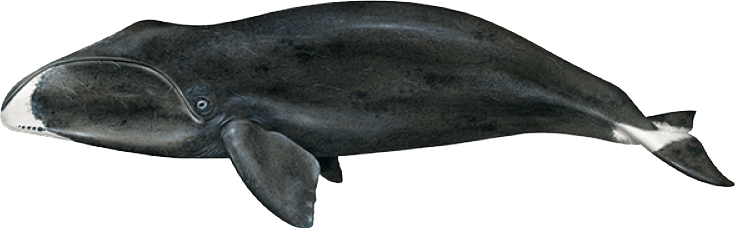
\includegraphics[width=0.50\linewidth]{Subject} \end{center}

\begin{center}
\includegraphics[width=0.50\linewidth]{logo} \end{center}

\newpage

\hypertarget{abstract}{%
\subsubsection{Abstract}\label{abstract}}

\hypertarget{introduction}{%
\subsubsection{Introduction}\label{introduction}}

\hypertarget{methods}{%
\subsubsection{Methods}\label{methods}}

\textbf{Data Collection} To observe bowhead whales, visual aerial
line-transect surveys were conducted in coast land offshore areas in
West Greenland between 65°400N and 75°300N, largely covering the area of
the local spring aggregation in Disko Bay. The study region on
242,650km\textsuperscript{2} was divided into 16 strata based on prior
knowledge of anticipated densities of bowhead whales. Between 24th March
and 14th April 2012 7,836.5km of total east-west oriented transect lines
were observed, with the targeted altitude and speed being 213m and 167
km/h respectively. Surveying was only carried out if Beaufort Sea States
Code was 2 or less, i.e.~only when the sea was calm. Inclinometers were
used to measure the angle of declination for each observed group of
bowhead whales (Suunto). The angles were then converted to perpendicular
distances (\(x\)) using the following equation from Buckland et
al.~(2001):

\(x = v * tan(90 - \psi )\),

where \(v\) is the altitude of the airplane, \(\psi\) is the declination
angle. Forward distance (\(y\)) to each sighting was calculated based on
time of first sighting, time when passing abeam and speed of aircraft.
For a more extensive description of the data collection refer to Rekdal
et al.~(2015).

\textbf{Distance Sampling} To estimate the abundance of bowhead whales,
a sample representative portion of the area, i.e.~the plot distance
sampling, is used. Distance sampling is used in ecological surveys to
account for imperfect detections and is incredibly useful considering
limited resources. The bowhead whales further away are less likely to be
detected, thus distance is employed as a detection bias. The detection
function describes how detectability varies with distance, it includes
the proportion of animals seen at a given distance and a probability of
seeing an animal at a given distance. To employ the distance sampling,
first of the assumptions need to be met: - the transect lines were
placed at random and the bowhead whales were not affected by their
placement; - animals on the transect line, in this case from distance
from the plane of XX were seen with probability p = 1; - perpendicular
distances from line to bowhead whales are uniform random variables π(x)
= 1/w; - distances were measured without error and to the initial
location.

\textbf{Data Analysis}\\
Due to an obscured view close to the transect line, detections were
left-truncated at 100m Rekdal et al.~(2015).\\
8 models were fit to the distance data using all combinations of
hazard-rate and half-normal detection functions with cosine, hermite
polynomial and simple polynomial adjustments. Model selection using
Akaike information criterion (AIC) found that the best model was a
half-normal with no adjustments (see figure 1). AICc was also applied
due to the ratio of model parameters to observation being less than 1:40
and found the same result (Takezawa, 2014). This model had an good fit;
Cramer-von Mises test (T = 0.073, p = 0.732), bootstrap
Kolmogorov-Smirnov test for goodness-of-fit (D = 0.073, p = 1).
Additionally a QQ-plot comparing empirical and fitted CDF had points
lying approximately on the 1:1 line (see figure 1).

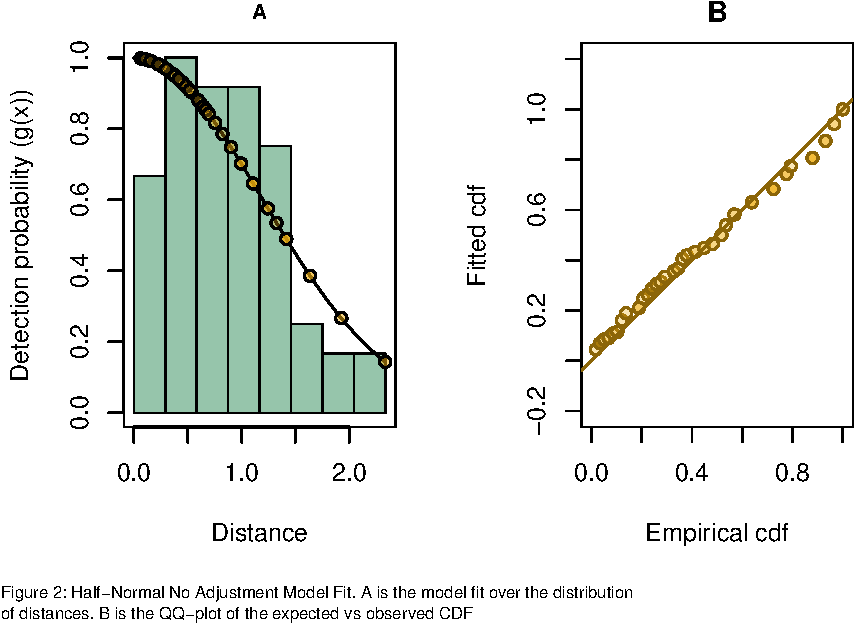
\includegraphics{Whale-Abundance_files/figure-latex/Model Fit Plot-1.pdf}

\hypertarget{results}{%
\subsubsection{Results}\label{results}}

\hypertarget{discussion}{%
\subsubsection{Discussion}\label{discussion}}

\hypertarget{references}{%
\subsubsection{References}\label{references}}

\hypertarget{appendix}{%
\subsubsection{Appendix}\label{appendix}}

R Analysis Code

\begin{Shaded}
\begin{Highlighting}[]
\DocumentationTok{\#\#\#\#\#    SETTING UP    \#\#\#\#\#}

\CommentTok{\# Set up packages }
\FunctionTok{library}\NormalTok{(Distance)}
\FunctionTok{library}\NormalTok{(tidyverse)}
\FunctionTok{library}\NormalTok{(remotes)}

\CommentTok{\# Getting Package Statsecol from github which contains the data}
\NormalTok{remotes}\SpecialCharTok{::}\FunctionTok{install\_github}\NormalTok{(}\StringTok{"https://github.com/chrissuthy/statsecol"}\NormalTok{)}

\CommentTok{\# Loading in the data package}
\FunctionTok{library}\NormalTok{(statsecol)}
\end{Highlighting}
\end{Shaded}

\begin{verbatim}
## 'data.frame':    84 obs. of  9 variables:
##  $ Region.Label: int  2 2 2 2 2 2 2 2 2 2 ...
##  $ Area        : int  8941 8941 8941 8941 8941 8941 8941 8941 8941 8941 ...
##  $ Sample.Label: int  3 3 4 4 4 4 4 4 4 4 ...
##  $ Effort      : num  98.8 98.8 181.4 181.4 181.4 ...
##  $ distance    : num  0.996 1.108 0.128 0.357 0.301 ...
##  $ y           : num  0.55 0.015 0.023 0.0025 0.57 0.51 0.34 0.091 0.029 0.021 ...
##  $ size        : num  1 1 1 1 1 2 2 1 2 2 ...
##  $ bf          : int  0 0 0 0 0 0 0 0 0 0 ...
##  $ object      : int  1 2 3 4 5 6 7 8 9 10 ...
\end{verbatim}

\includegraphics{Whale-Abundance_files/figure-latex/Exploratory Analysis-1.pdf}

\begin{Shaded}
\begin{Highlighting}[]
\DocumentationTok{\#\#\#\#\#     MODELLING     \#\#\#\#\#}

\CommentTok{\# Due to the long shoulder seen in the histogram, first fit a hazard rate;}
\CommentTok{\#   then fit a half{-}normal}


\CommentTok{\# Fitting hazard{-}rate detection functions with all adjustment terms }

\CommentTok{\# Hazard{-}rate with no adjustment }
\NormalTok{hr }\OtherTok{\textless{}{-}} \FunctionTok{ds}\NormalTok{(}\AttributeTok{data =}\NormalTok{ bowhead\_LT, }
         \AttributeTok{key =} \StringTok{"hr"}\NormalTok{, }
         \AttributeTok{adjustment =} \ConstantTok{NULL}\NormalTok{ ) }

\CommentTok{\# Hazard{-}rate with a cosine adjustment }
\NormalTok{hr\_cos }\OtherTok{\textless{}{-}} \FunctionTok{ds}\NormalTok{(}\AttributeTok{data =}\NormalTok{ bowhead\_LT, }
             \AttributeTok{key =} \StringTok{"hr"}\NormalTok{, }
             \AttributeTok{adjustment =} \StringTok{"cos"}\NormalTok{)}

\CommentTok{\# Hazard{-}rate with a hermite polynomial adjustment }
\NormalTok{hr\_herm }\OtherTok{\textless{}{-}} \FunctionTok{ds}\NormalTok{(}\AttributeTok{data =}\NormalTok{ bowhead\_LT, }
              \AttributeTok{key =} \StringTok{"hr"}\NormalTok{, }
              \AttributeTok{adjustment =} \StringTok{"herm"}\NormalTok{ )}

\CommentTok{\# Hazard{-}rate with a simple polynomial adjustment }
\NormalTok{hr\_poly }\OtherTok{\textless{}{-}} \FunctionTok{ds}\NormalTok{(}\AttributeTok{data =}\NormalTok{ bowhead\_LT, }
              \AttributeTok{key =} \StringTok{"hr"}\NormalTok{, }
              \AttributeTok{adjustment =} \StringTok{"poly"}\NormalTok{ ) }



\CommentTok{\# Fitting half{-}normal detection functions with all adjustment terms }

\CommentTok{\# Half{-}normal with no adjustment }
\NormalTok{hn }\OtherTok{\textless{}{-}} \FunctionTok{ds}\NormalTok{(}\AttributeTok{data =}\NormalTok{ bowhead\_LT, }
         \AttributeTok{key =} \StringTok{"hn"}\NormalTok{, }
         \AttributeTok{adjustment =} \ConstantTok{NULL}\NormalTok{ ) }

\CommentTok{\# Half{-}normal with a cosine adjustment}
\NormalTok{hn\_cos }\OtherTok{\textless{}{-}} \FunctionTok{ds}\NormalTok{(}\AttributeTok{data =}\NormalTok{ bowhead\_LT, }
             \AttributeTok{key =} \StringTok{"hn"}\NormalTok{, }
             \AttributeTok{adjustment =} \StringTok{"cos"}\NormalTok{ ) }

\CommentTok{\# Half{-}normal with a hermite polynomial adjustment}
\NormalTok{hn\_herm }\OtherTok{\textless{}{-}} \FunctionTok{ds}\NormalTok{(}\AttributeTok{data =}\NormalTok{ bowhead\_LT, }
              \AttributeTok{key =} \StringTok{"hn"}\NormalTok{, }
              \AttributeTok{adjustment =} \StringTok{"herm"}\NormalTok{ )}

\CommentTok{\# Half{-}normal with a simple polynomial adjustment}
\NormalTok{hn\_poly }\OtherTok{\textless{}{-}} \FunctionTok{ds}\NormalTok{(}\AttributeTok{data =}\NormalTok{ bowhead\_LT, }
              \AttributeTok{key =} \StringTok{"hn"}\NormalTok{, }
              \AttributeTok{adjustment =} \StringTok{"poly"}\NormalTok{ )}
\end{Highlighting}
\end{Shaded}

\begin{Shaded}
\begin{Highlighting}[]
\DocumentationTok{\#\#\#\#\#     MODEL SELECTION     \#\#\#\#\#}

\CommentTok{\# Comparing Models graphically by fit of detection probability over distance distribution}

\CommentTok{\# Half{-}normal detection function over histogram plot}
\CommentTok{\# Setting up plot size and margins}
\FunctionTok{par}\NormalTok{(}\AttributeTok{mfrow =} \FunctionTok{c}\NormalTok{(}\DecValTok{2}\NormalTok{, }\DecValTok{2}\NormalTok{), }
    \AttributeTok{mar =} \FunctionTok{c}\NormalTok{(}\DecValTok{5}\NormalTok{, }\DecValTok{4}\NormalTok{, }\DecValTok{4}\NormalTok{, }\DecValTok{2}\NormalTok{) }\SpecialCharTok{+} \FloatTok{0.1}\NormalTok{) }

\CommentTok{\# Plotting all 4 half{-}normal models}
\FunctionTok{plot}\NormalTok{(hn, }\AttributeTok{main =} \StringTok{"no adjustment"}\NormalTok{) }
\FunctionTok{plot}\NormalTok{(hn\_cos, }\AttributeTok{main =} \StringTok{"cosine"}\NormalTok{)}
\FunctionTok{plot}\NormalTok{(hn\_poly, }\AttributeTok{main =} \StringTok{"polynomial"}\NormalTok{)}
\FunctionTok{plot}\NormalTok{(hn\_herm, }\AttributeTok{main =} \StringTok{"hermite polynomial"}\NormalTok{)}
\FunctionTok{title}\NormalTok{(}\StringTok{"Half{-}Normal Models"}\NormalTok{, }
      \AttributeTok{line =} \SpecialCharTok{{-}}\DecValTok{1}\NormalTok{, }
      \CommentTok{\# Naming title and setting location}
      \AttributeTok{outer =} \ConstantTok{TRUE}\NormalTok{) }


\CommentTok{\# Hazard{-}rate Detection function over histogram plot}
\FunctionTok{par}\NormalTok{(}\AttributeTok{mfrow =} \FunctionTok{c}\NormalTok{(}\DecValTok{2}\NormalTok{, }\DecValTok{2}\NormalTok{), }
    \CommentTok{\# Setting up plot size and margins}
    \AttributeTok{mar =} \FunctionTok{c}\NormalTok{(}\DecValTok{5}\NormalTok{, }\DecValTok{4}\NormalTok{, }\DecValTok{4}\NormalTok{, }\DecValTok{2}\NormalTok{) }\SpecialCharTok{+} \FloatTok{0.1}\NormalTok{) }

\CommentTok{\# Plotting all 4 hazard{-}rate models}
\FunctionTok{plot}\NormalTok{(hr, }\AttributeTok{main =} \StringTok{"no adjustment"}\NormalTok{)}
\FunctionTok{plot}\NormalTok{(hr\_cos, }\AttributeTok{main =} \StringTok{"cosine"}\NormalTok{)}
\FunctionTok{plot}\NormalTok{(hr\_poly, }\AttributeTok{main =} \StringTok{"polynomial"}\NormalTok{)}
\FunctionTok{plot}\NormalTok{(hr\_herm, }\AttributeTok{main =} \StringTok{"hermite polynomial"}\NormalTok{)}
\FunctionTok{title}\NormalTok{(}\StringTok{"Hazard{-}Rate Models"}\NormalTok{, }
      \AttributeTok{line =} \SpecialCharTok{{-}}\DecValTok{1}\NormalTok{, }
      \CommentTok{\# Naming title and setting location}
      \AttributeTok{outer =} \ConstantTok{TRUE}\NormalTok{) }

\CommentTok{\# Comparing AIC of all the models }
\FunctionTok{summarize\_ds\_models}\NormalTok{(hn, hn\_cos, hn\_herm, hn\_poly, }
\NormalTok{                    hr, hr\_cos, hr\_herm, hr\_poly,}
                    \CommentTok{\# Plain output works instead of equations}
                    \AttributeTok{output =} \StringTok{"plain"}\NormalTok{) }

\CommentTok{\# As the dataset is small, checking whether AICc is a more appropriate measure}
\CommentTok{\# To do this, Takezawa (2014) has said AICc should be used when the ratio of your parameters}
\CommentTok{\#   to number of data points is less than 1:40}
\CommentTok{\# Print summary of hazard{-}rate distance model}
\FunctionTok{summary}\NormalTok{(hr)}
  \CommentTok{\# Parameters = 2 : Observations = 58}
  \CommentTok{\# Therefore ratio is 1:29}
  \CommentTok{\#   This ratio will be even smaller for the models with adjustments }

\CommentTok{\# Print summary of half{-}normal distance model}
\FunctionTok{summary}\NormalTok{(hn)}
  \CommentTok{\# This is the only model that meets the assumptions of AIC however as you }
  \CommentTok{\#   Can"t compare across model selection parameters we will use AICc}

\CommentTok{\# Using AICc to select models }
\FunctionTok{AICc}\NormalTok{(hn, hn\_cos, hn\_herm, hn\_poly, }
\NormalTok{     hr, hr\_cos, hr\_herm, hr\_poly)}

\CommentTok{\# Despite this there is no change in the best model}

\CommentTok{\# The half{-}normal will be chosen as it has the smallest AIC and AICc}
\CommentTok{\# No adjustment will be chosen as the adjustments don"t model extra variability }
\CommentTok{\#   in the data }
\end{Highlighting}
\end{Shaded}

\begin{Shaded}
\begin{Highlighting}[]
\DocumentationTok{\#\#\#\#\#     MODEL FIT     \#\#\#\#\#}

\CommentTok{\# Comparing the detection function to the cramer{-}von mises test}

\CommentTok{\# Setting plot size}
\FunctionTok{par}\NormalTok{(}\AttributeTok{mfrow =} \FunctionTok{c}\NormalTok{(}\DecValTok{1}\NormalTok{,}\DecValTok{2}\NormalTok{), }\AttributeTok{mar =} \FunctionTok{c}\NormalTok{(}\DecValTok{5}\NormalTok{, }\DecValTok{4}\NormalTok{, }\DecValTok{4}\NormalTok{, }\DecValTok{2}\NormalTok{) }\SpecialCharTok{+} \FloatTok{0.1}\NormalTok{)}

\CommentTok{\# Plotting the detetion function over the distances distribution}
\FunctionTok{plot}\NormalTok{(hn, }
     \AttributeTok{which =} \DecValTok{2}\NormalTok{, }
     \AttributeTok{pl.col =} \FunctionTok{adjustcolor}\NormalTok{(}\StringTok{"seagreen"}\NormalTok{, }\FloatTok{0.5}\NormalTok{), }
     \AttributeTok{border =} \ConstantTok{NULL}\NormalTok{,}
     \AttributeTok{ylab =} \StringTok{"Detection probability (g(x))"}\NormalTok{, }
     \AttributeTok{xlab =} \StringTok{"Distance"}\NormalTok{, }
     \AttributeTok{las =} \DecValTok{1}\NormalTok{,}
     \AttributeTok{main =} \StringTok{"Half{-}normal Model No Adjustments"}\NormalTok{)}

\CommentTok{\# Plotting and running the Cramer{-}von Mises test and bootstrap Kolmogorov{-}Smirnov      }
\CommentTok{\#   test for goodness{-}of{-}fit}

\FunctionTok{gof\_ds}\NormalTok{(hn, }\AttributeTok{main =} \StringTok{"Expected vs Observed CDF"}\NormalTok{, }\AttributeTok{ks =} \ConstantTok{TRUE}\NormalTok{)}

  \CommentTok{\# The Cramer{-}von Mises test gives a test statistic of 0.0732325 and a p{-}value }
  \CommentTok{\#   of 0.731882}
  \CommentTok{\# The Kolomogorov{-}Smirnov test gives a test statistic stat of 0.0725551 and a             }
  \CommentTok{\#   p{-}value of 1}

\CommentTok{\# Therefore the model has a good fit as the p values are much more than 0.05}
\end{Highlighting}
\end{Shaded}

\begin{Shaded}
\begin{Highlighting}[]
\DocumentationTok{\#\#\#\#\#     MODEL INFERENCE     \#\#\#\#\#}
\CommentTok{\# Print summary of the model}
\FunctionTok{summary}\NormalTok{(hn)}

\CommentTok{\# Creating subsets of the column combinations needed for dht() density and }
\CommentTok{\#   abundance estimate and variances function.}
\CommentTok{\# Region labels and areas. }
\NormalTok{region\_table }\OtherTok{\textless{}{-}} \FunctionTok{unique}\NormalTok{(bowhead\_LT[, }\FunctionTok{c}\NormalTok{(}\StringTok{"Region.Label"}\NormalTok{, }
                                      \StringTok{"Area"}\NormalTok{)])}

\CommentTok{\# Region and sample labels, effort}
\NormalTok{sample\_table }\OtherTok{\textless{}{-}} \FunctionTok{unique}\NormalTok{(bowhead\_LT[, }\FunctionTok{c}\NormalTok{(}\StringTok{"Region.Label"}\NormalTok{, }
                                      \StringTok{"Sample.Label"}\NormalTok{, }
                                      \StringTok{"Effort"}\NormalTok{)])}

\CommentTok{\# Object, region and sample labels}
\NormalTok{observation\_table }\OtherTok{\textless{}{-}} \FunctionTok{unique}\NormalTok{(bowhead\_LT[, }\FunctionTok{c}\NormalTok{(}\StringTok{"object"}\NormalTok{, }
                                           \StringTok{"Region.Label"}\NormalTok{, }
                                           \StringTok{"Sample.Label"}\NormalTok{)])}

\CommentTok{\# Estimating bowhead whale abundance and density}
\NormalTok{abund\_bio\_hn }\OtherTok{\textless{}{-}} \FunctionTok{dht}\NormalTok{(}\AttributeTok{model =}\NormalTok{ hn}\SpecialCharTok{$}\NormalTok{ddf,}
\NormalTok{                    region\_table, }
\NormalTok{                    sample\_table, }
\NormalTok{                    observation\_table)}
\end{Highlighting}
\end{Shaded}


\end{document}
